\chapter{Risultati}
In questo capitolo, ci si è occupati di eseguire i test delle metriche sul Wi-Fi Direct, in due tipologie ambientali: Indoor e Outdoor. 
Nei test eseguiti, è stato riscontrato che nel caso outdoor, i due smartphone hanno una portata di ricezione massima fino a 80 metri, mentre nei test indoor fino a 20 metri.
\newpage

\section{Analisi 1: Packet Delivery Ratio}

Ambiente Indoor:
\begin{center}
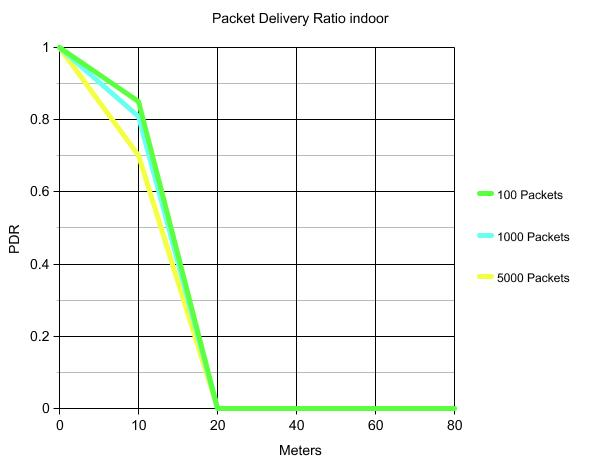
\includegraphics[width=1\textwidth]{imgs/PDR_Indoor_New.jpg}
\captionof{figure}{Rappresentazione in percentuale invio e ricezione pacchetti ambiente Indoor}\label{pdr_indoor_img}%
\end{center}

Come possiamo notare dalla figura \ref{pdr_indoor_img}, nell'asse delle ordinate sono stati posti i valori del range di distanza tra i due dispositivi misurati in metri, mentre nelle ordinate la percentuale di pacchetti che viene trasmessa e ricevuta.
Abbiamo analizzato 3 campioni composti rispettivamente da: 100, 1000 e 5000 pacchetti.
Si noti come all'aumentare della distanza la percentuale dei pacchetti trasmessi e ricevuti cali drasticamente fino ad arrivare a 0 raggiunti i 20 metri, ciò è causato anche dalla presenza di ostacoli ( muri ) avendo compiuto l'esperimento all'interno di una struttura.

Ambiente Outdoor:
\begin{center}
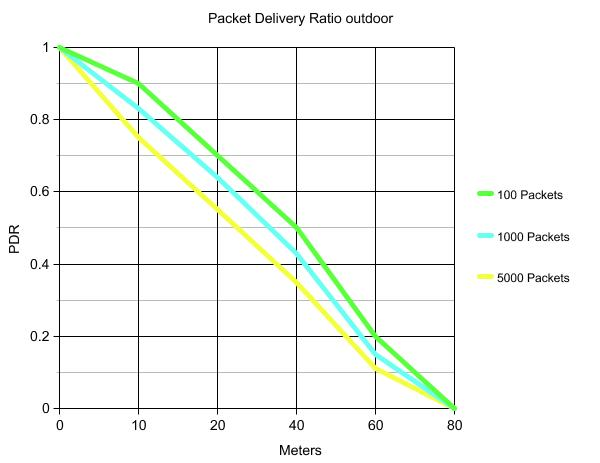
\includegraphics[width=1\textwidth]{imgs/PDR_Outdoor_New.jpg}
\captionof{figure}{Rappresentazione in percentuale invio e ricezione pacchetti ambiente Outdoor}\label{pdr_outdoor_img}%
\end{center}

Nel caso dell'ambiente outdoor, possiamo notare in figura \ref{pdr_outdoor_img} come invece la situazione tenda a migliorare, riuscendo a raggiungere una distanza di trasferimento e ricezione massima di 80 metri.
Nel caso outdoor è stata prestata molta attenzione nell'eseguire i test senza alcun tipo di ostacolo tra i due dispositivi.
\newpage

\section{Analisi 2: Throughput}

Ambiente Indoor:
\begin{center}
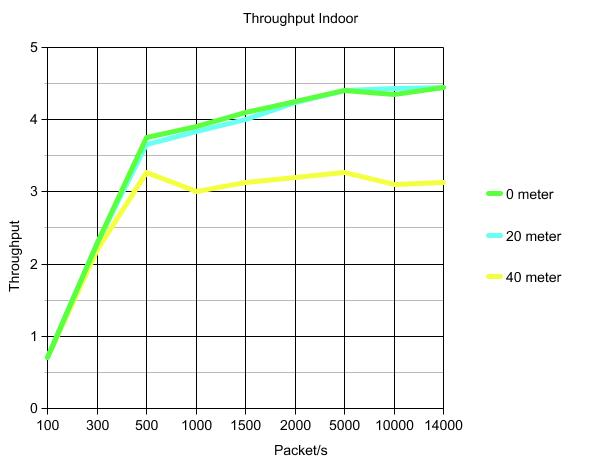
\includegraphics[width=1\textwidth]{imgs/ThroughputIndoor.jpg}
\captionof{figure}{Rappresentazione in Megabit (Mb) della quantità massima di dati inviabili in ambiente Indoor}\label{throughputindoor_img}%
\end{center}

Come possiamo notare nella figura \ref{throughputindoor_img}, nell'asse delle ordinate sono stati posti i valori che indicano il numero di pacchetti inviati da un dispositivo ad un altro fino ad un massimo di 14000, in quello delle ascisse invece la quantità di dati trasmessa in Megabit (Mb) fino ad un massimo di 5.
Ogni linea del grafico rappresenta una distanza diversa tra i dispositivi, rispettivamente: 0 metri, 10 metri e 20 metri.
Si noti come non si superino i 5Mb e nel caso dell'ultima linea di distanza (20 metri) come sia presente una perdita significativa di byte, mentre invece nel caso delle altre 2 come convergano nel medesimo punto.

Ambiente Outdoor:
\begin{center}
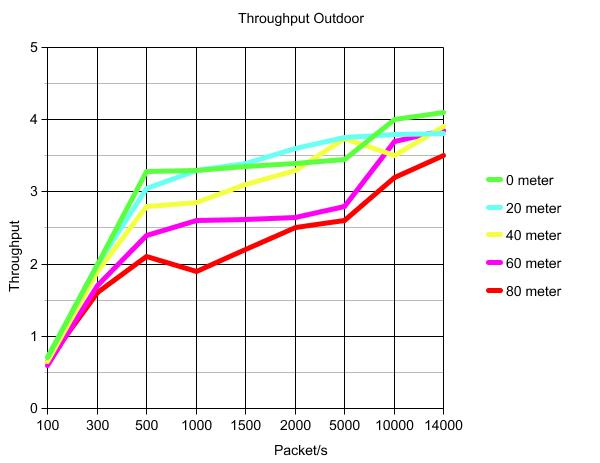
\includegraphics[width=1\textwidth]{imgs/ThroughputOutdoor.jpg}
\captionof{figure}{Rappresentazione in Megabit (Mb) della quantità massima di dati inviabili in ambiente Indoor}\label{throughputoutdoor_img}%
\end{center}

Come possiamo notare nella figura \ref{throughputoutdoor_img} anche nel caso outdoor non si superano i 5 Mb, ma si noti anche come le linee che rappresentano rispettivamente le distanze: 0, 20, 40, 60 e 80 metri convergano quasi negli stessi punti, fatta eccezione per gli 80 metri in cui si comincia ad intravedere una discreta perdita di Byte.

\section{Analisi 3: Discovery Time}
Come detto in precedenza, per tale metrica sono stati effettuati 2 tipi di test diversi con più dispositivi: 

-Discovery Time without Group Owner
-Discovery Time with Group Owner

\subsection{Discovery Time without Group Owner (GO)}

Ambiente Indoor:
\begin{center}
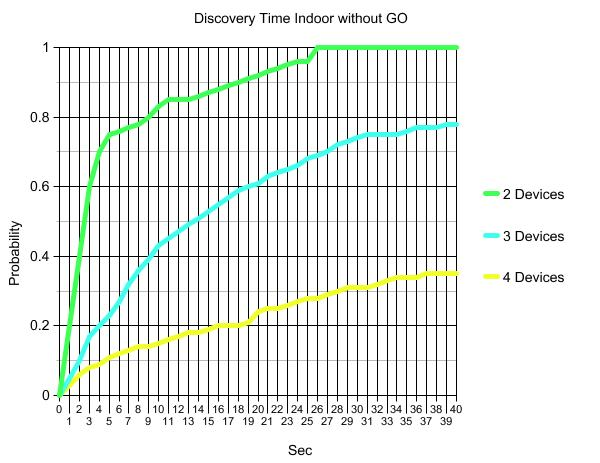
\includegraphics[width=1\textwidth]{imgs/Discovery_Time_Indoor_no_GO.jpg}
\captionof{figure}{Rappresentazione tempo associazione tra più dispositivi senza Group Owner in ambiente Indoor}\label{discoverytimeindoornogo_img}%
\end{center}

Nella figura \ref{discoverytimeindoornogo_img} è stato rappresentata in percentuale la probabilità di associazione tra più dispositivi, ponendo nelle asse delle ordinate i secondi impiegati e nelle asse delle ascisse la percentuale.
Da tale grafico si può notare come due dispositivi abbiamo probabilità molto alta di completare con successo l'associazione diventando certa dopo un tempo di 26 secondi.
Caso diverso invece per quanto riguarda l'associazione tra 3 e 4 dispositivi presentado una probabilità alquanto bassa, nel caso di 3 dispositivi dopo i 40 secondi siamo ancora su una probabilità di 0.8, mentre invece nel caso di 4 dispositivi siamo sullo 0.4.

Ambiente Outdoor:
\begin{center}
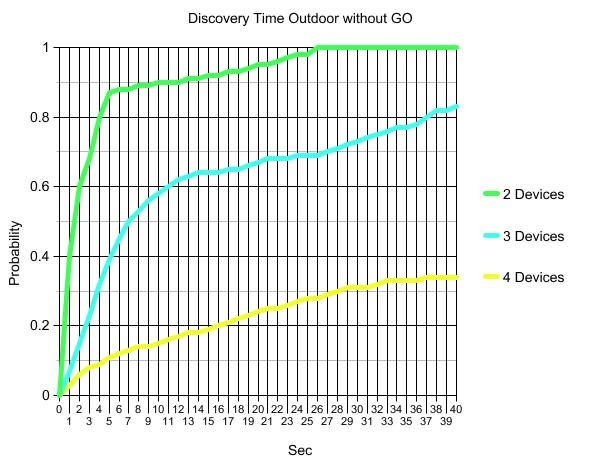
\includegraphics[width=1\textwidth]{imgs/Discovery_Time_Outdoor_no_GO.jpg}
\captionof{figure}{Rappresentazione tempo associazione tra più dispositivi senza Group Owner in ambiente Outdoor}\label{discoverytimeoutdoornogo_img}%
\end{center}

Nella figura \ref{discoverytimeoutdoornogo_img} si nota invece un discreto miglioramento per quanto riguarda l'associazione tra 2 e 3 dispositivi, mentre invece la situazione rimane tale per il caso dei 4 dispositivi.
\newpage

\subsection{Discovery Time with Group Owner (GO)}

Ambiente Indoor:
\begin{center}
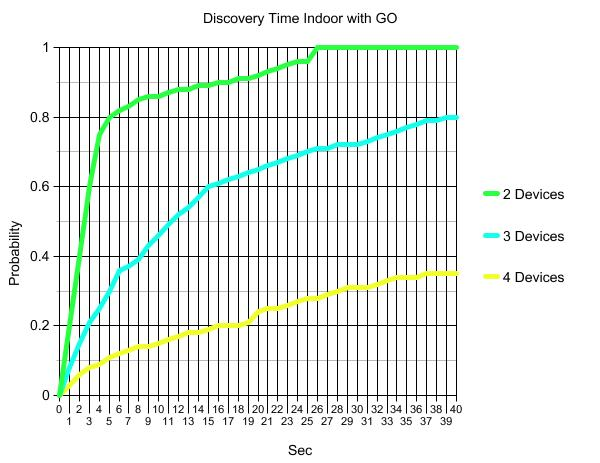
\includegraphics[width=1\textwidth]{imgs/Discovery_Time_Indoor_with_GO.jpg}
\captionof{figure}{Rappresentazione tempo associazione tra più dispositivi senza Group Owner in ambiente Outdoor}\label{discoverytimeindoorwithgo_img}%
\end{center}

Come possiamo notare dalla figura \ref{discoverytimeindoorwithgo_img}, possiamo notare miglioramenti rispetto al test di prima con una probabilità di successo di associazione di 0.8 a 5 secondi per 2 dispositivi, mentre invece di 0.6 a 15 secondi per 3 dispositivi, per il caso di 4 dispositivi invece si rimane sempre sullo 0.4.
\newpage

Ambiente Outdoor:
\begin{center}
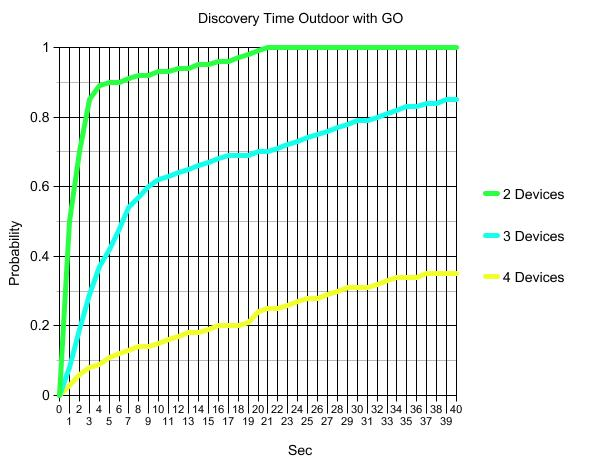
\includegraphics[width=1\textwidth]{imgs/Discovery_Time_Outdoor_with_GO.jpg}
\captionof{figure}{Rappresentazione tempo associazione tra più dispositivi senza Group Owner in ambiente Outdoor}\label{discoverytimeoutdoorwithgo_img}%
\end{center}

Dalla figura \ref{discoverytimeoutdoorwithgo_img}, possiamo notare che anche nel caso Outdoor si sono presentati notevoli miglioramenti, con una probabilità di successo di 0.9 a 5 secondi per il caso di 2 dispositivi, sempre una probabilità di successo dello 0.6 ma stavolta a 9 secondi, mentre invece per il caso di 4 dispositivi rimane sempre allo 0.4.
\newpage

Quindi, riassumendo tutti e 4 i grafici in uno solo:
\begin{center}
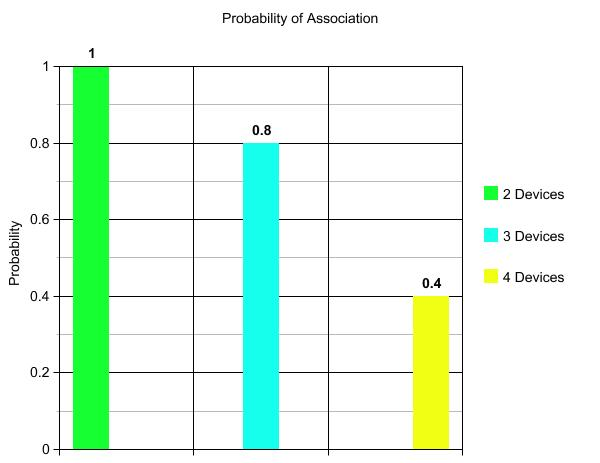
\includegraphics[width=1\textwidth]{imgs/probability_of_association.jpg}
\captionof{figure}{Rappresentazione tempo associazione tra più dispositivi senza Group Owner in ambiente Outdoor}\label{probabilityofassociation_img}%
\end{center}

In conclusione si può notare che la probabilità di associazione tra 2 dispositivi è pari ad 1 (quindi una certezza), mentre invece per il caso di 3 dispositivi o 4 dispositivi la probabilità massima è rispettivamente di 0.6 e 0.4.

\clearpage{\pagestyle{empty}\cleardoublepage}